\documentclass[wi]{zut}

\usepackage{microtype}
\usepackage{wrapfig}

\author{Karol Działowski}
\title{Pytania na obronę pracy magisterskiej}

\makemetadata

\begin{document}

\maketitle
\tableofcontents

\section{Wstęp}

Poniższe opracowania były opracowywane indywidualnie i nie są oficjalnymi ani sprawdzonymi odpowiedziami na pytania. Na wiele pytań nie jestem pewien udzielonej odpowiedzi -- przy nich widnieje znak zapytania jak na przykładzie niżej.

W tym akapicie przedstawiony jest schemat oznaczenia pytań co do których odpowiedzi nie mam pewności. Po prawej stronie będzie wklejona ikona znaku zapytania.
\question

Podczas opracowywania pytań starałem się tłumaczyć możliwie jak najogólniej powiązane zagadnienia. W wielu przypadkach też zamieściłem odnośniki do źródeł z których korzystałem podczas tworzenia z tego dokumentu.

Zachęcam do składania poprawek poprzez stworzenie pull-requestów na repozytorium, które dostępne jest pod adresem \url{https://github.com/karlosos/ZUT_pytania_magisterskie}.

\section{Przedmioty wspólne}

% \subsection{Zasady cyfryzacji sygnałów. Prawo Kotielnikowa-Shannona. Granica Nyquisa. Aliasing.}
% TODO
% Aleksandr Cariow. Cyfrowe przetwarzanie sygnałów.

% \subsection{Bezpieczny schemat podpisu cyfrowego. Modele bezpieczeństwa.}
% TODO
% Tomasz Hyla. Kryptologia.

% \subsection{Idea interpolacji funkcji z wykorzystaniem funkcji sklejanych.}
% TODO
% Piotr Piela. Matematyka obliczeniowa.

% \subsection{Styl poznawczy (kognitywny) człowieka}
% TODO
% Izabela Rejer. Wprowadzenie do kognitywistyki.

% \subsection{Korzyści wynikające z zastosowania grafowych baz danych do przetwarzania dużych zbiorów danych o strukturach grafowych}
% TODO
% Przemysław Korytkowski. Duże zbiory danych.

% \subsection{Założenia i obszary zastosowania platformy Apache Spark}
% TODO
% Przemysław Korytkowski. Duże zbiory danych.

\subsection{Sposoby sprawdzenia właściwości losowych danego ciągu}
% Tomasz Hyla. Kryptologia.

Testy generatorów ciągów losowych:

\begin{itemize}
    \item Test pojedynczych bitów - monobit test
    \item Test ,,pokerowy''
    \item Test ,,długich podciągów identycznych ciągów''
    \item Test ,,podciągów identycznych ciągów''
    \item Dieharder
    \item NIST Statistical Test Suite \cite{Chocian2020_2}
\end{itemize}

\paragraph{Test pojedynczych bitów - \emph{monobit test}}

Wygenerować ciąg binarny o długości 20000 bitów. \textbf{Należy określić liczbę $X$ wszystkich bitów o wartości $1$ występujących w badanym ciągu.} Wynik testu jest pomyślny gdy, $9725 < X < 10275$.

\paragraph{Test ,,pokerowy''}

Wygenerować ciąg binarny o długości 20000 bitów. \textbf{Podzielić badany ciąg na 4-bitowe paczki obejmujące 4 kolejne bity (takich paczek jest 5000)}. Zliczyć częstości $f(i)$ pojawiania się każdej z możliwych 16 sekwencji bitowych. Obliczyć wielkość $X = (16/5000) \sum{f(i)^2} - 5000$. Wynik testu jest pomyślny, gdy $2.16 < X < 46.17$.

\paragraph{Test ,,długich podciągów identycznych ciągów'' (Long runs test)}

Wygenerować ciąg binarny o długości 20000 bitów.  Jeżeli w badanym ciągu istnieje co najmniej jeden podciąg o długości $>26$ bitów zaweirający same 0 lub same 1, to wynik testu jest negatywny.

\paragraph{Test ,,podciągów identycznych ciągów'' (Runs test)}

Zliczyć wszystkie podciągi składające się tylko z bitów o wartości 0, albo tylko z bitów o wartości 1. Podzielić te podciągi na 6 grup: pierwszą - zawierającą podciągi u długości 1 bita, drugą - zawierającą podciągi o długości 2 bitów, itd.

Jeżeli liczebność którejkolwiek z sześciu grup podciągów nie mieści się w zakresie podanym w tablicy, to wynik testu jest negatywny~\cite{Chocian2020_2}.

\begin{table}[H]
\centering
\begin{tabular}{@{}rc@{}}
\toprule
Indeks paczki & Zakres    \\ \midrule
1             & 2315-2685 \\
2             & 1114-1386 \\
3             & 527-723   \\
4             & 240-384   \\
5             & 103-209   \\
6+            & 103-209   \\ \bottomrule
\end{tabular}
\end{table}

% TODO opisać wszystkie testy

% \subsection{Filtracja cyfrowa: filtry SOI i NOI}
% TODO
% Aleksandr Cariow. Cyfrowe przetwarzanie sygnałów.

% \subsection{Reprezentacja sygnałów za pomocą szeregów funkcyjnych. Dyskretne transformacje ortogonalne oraz szybkie algorytmy ich wyznaczania.}
% TODO
% Aleksandr Cariow. Cyfrowe przetwarzanie sygnałów.

\subsection{Atak na podpis cyfrowy wykorzystujący paradoks dnia urodzin}
% Tomasz Hyla. Kryptologia.

Paradoks dnia urodzin odnosi się do prawdopodobieństwa tego, że w zbiorze $n$ losowo wybranych ludzi będzie para, która ma urodziny tego samego dnia. W grupie liczącej 23 osoby to prawdopodobieństwo wynosi 50\%, a grupa 70 osób ma 99.9\% prawdopodobieństwa występowania takiej pary \cite{wiki:Birthday_problem}.


\begin{figure}[H]
    \centering
    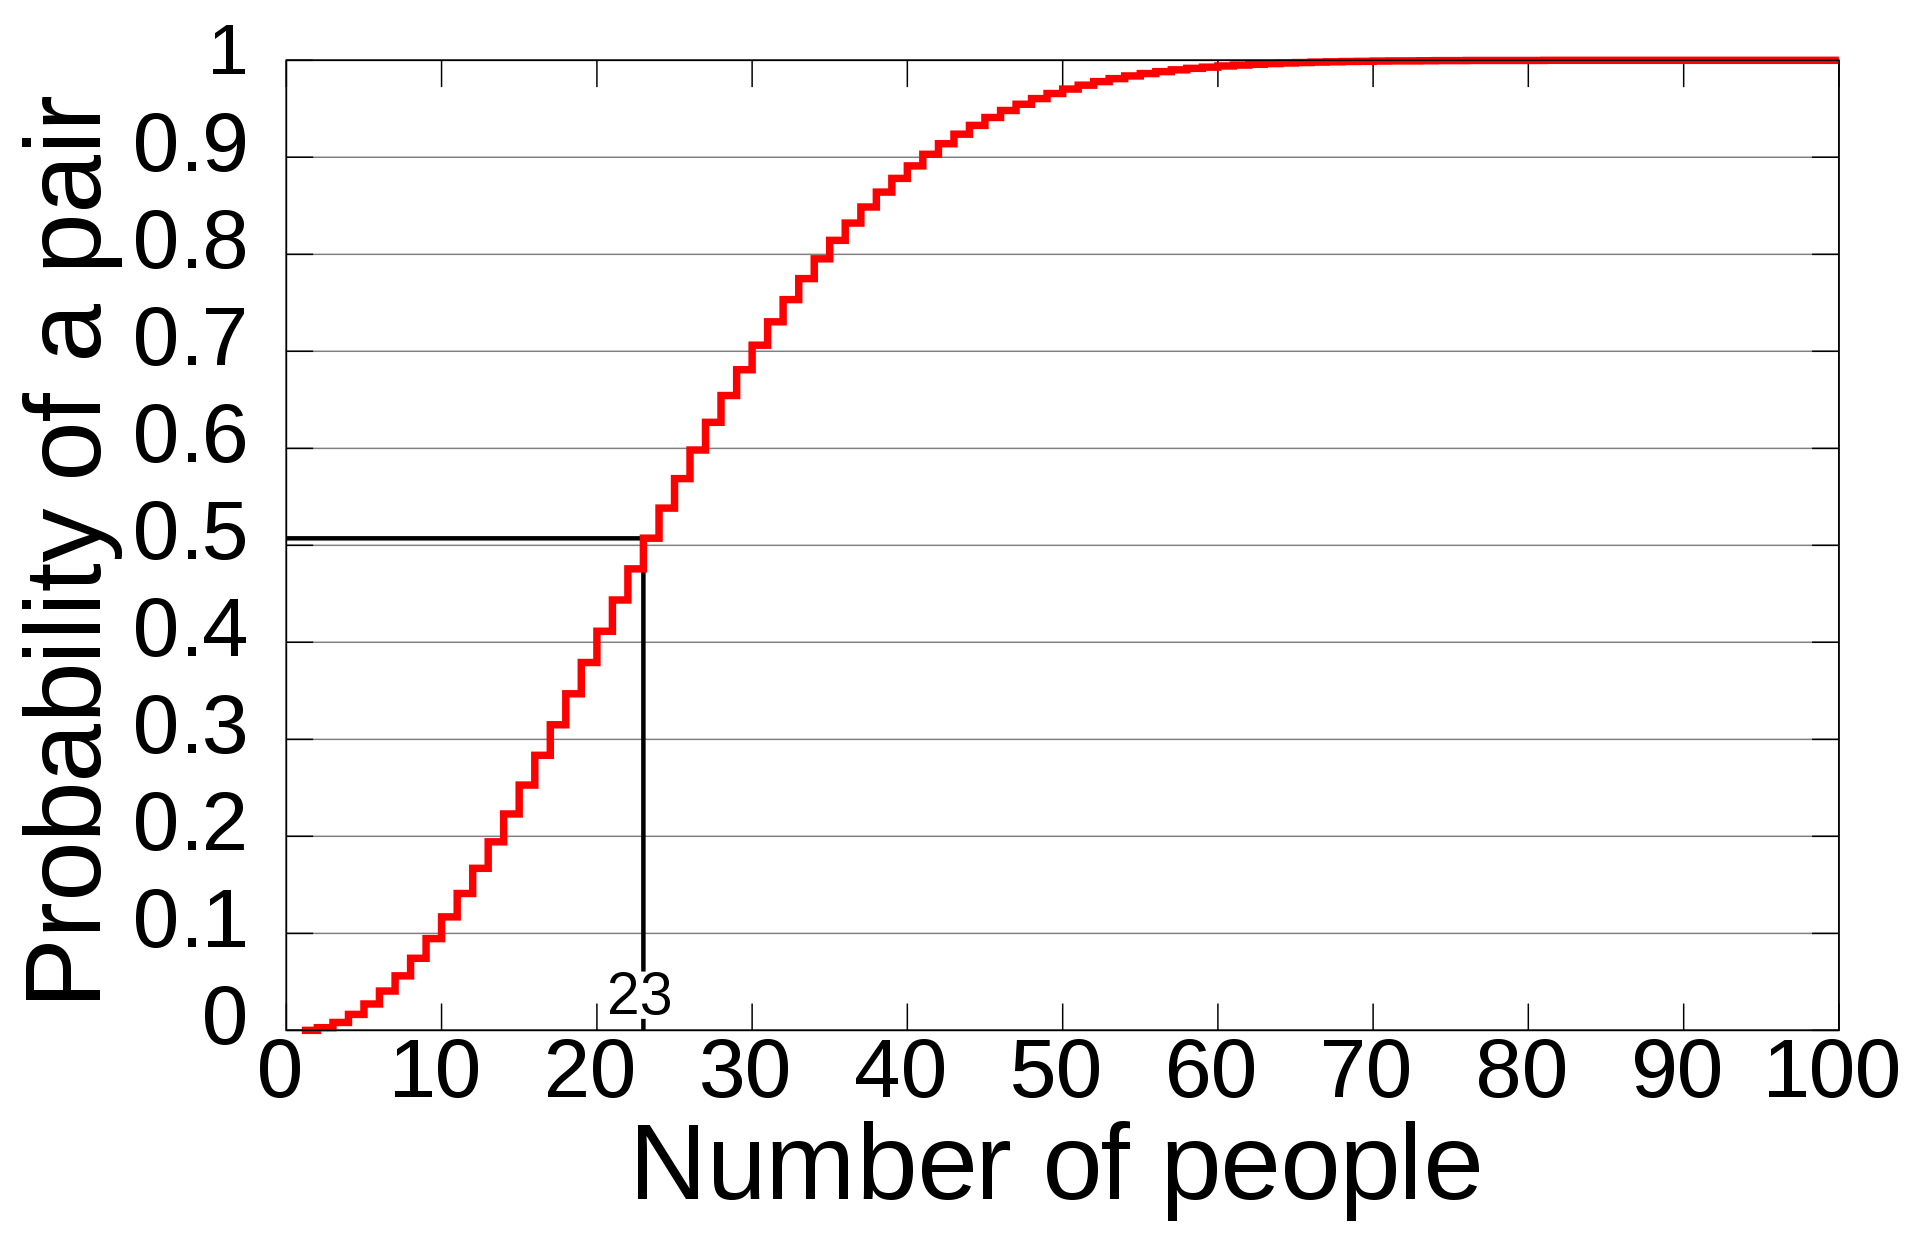
\includegraphics[width=0.5\linewidth]{images/Birthday_Paradox.svg.png}
    %\vspace{1em}
    \caption{Obliczone prawdopodobieństwo, ze co najmniej dwie osoby mają wspólną datę urodzenia.}
    \label{fig:birthdaj}
    \source{\url{https://www.wikiwand.com/en/Birthday_problem} \cite{wiki:Birthday_problem}}
\end{figure}

Podpisy cyfrowe mogą być podatne na atak wykorzystujący paradoks dnia urodzin (ang. birthday attack). Zazwyczaj podpisywanie wiadomości $m$ zaczyna się od obliczenia $f(m)$, gdzie $f$ to kryptograficzna funkcja skrótu a następnie używa się tajnego klucza do podpisu $f(m)$ (wartości skrótu z wiadomości). Załóżmy że adwersarz, chce wrobić Boba w podpis nieuczciwego dokumentu. Adwersarz przygotowuje uczciwy dokument $m$ i nieuczciwy $m'$. Uczciwy dokument $m$ jest tak modyfikowany (np. dodawane białe znaki) aby jego skrót był równy skrótowy z dokumentu $m'$, czyli $f(m) = f(m')$~\cite{wiki:Birthday_problem}.

W takiej sytuacji, gdy Bob podpisze dokument $m$ będzie to równoważne z podpisaniem $m'$.

Aby obronić się przed tym atakiem, długość skrótu powinna być stosunkowo duża, aby znalezienie kolizji było wystarczająco trudne. Innym sposobem na przeciwdziałanie temu atakowi, jest mała zmiana dokumentu przez Boba przed podpisaniem (ale wtedy adwersarz może tak samo szukać kolizji zmieniając fałszywy dokument)~\cite{wiki:Birthday_problem}.

Na wykładach atak ten był przedstawiony w trochę inny sposób. Podpis cyfrowy dla wiadomości $m$ to $s = D_d(h(m))$, gdzie $D_d$ to klucz prywatny Boba, $h$ to funkcja skrótu. Mając skrót o długości $n$ bitów należy:

\begin{itemize}
    \item wygenerować $2^{n/2}$ fałszywych wiadomości $m_i$
    \item wygenerować $2^{n/2}$ fałszywych podpisów $s_i$
    \item znaleźć taką parę, że $E_e(s_j) = h(m_k)$, gdzie $E$ to klucz publiczny Boba \cite{Chocian2020}.
\end{itemize}

% \subsection{Podział metod rozwiązywania równań liniowych metodami numerycznymi}
% TODO
% Piotr Piela. Matematyka obliczeniowa.

% \subsection{Algorytm numeryczny niestabilny a algorytm źle uwarunkowany}
% TODO
% Piotr Piela. Matematyka obliczeniowa.

% \subsection{Programowanie kodu wielowątkowego wraz z wzajemnym wykluczaniem w C++ 11 Threads}
% TODO
% Marek Pałkowski. Obliczenia dużej mocy.

% \subsection{Cechy środowiska Hadoop}
% TODO
% Przemysław Korytkowski. Duże zbiory danych.

% \subsection{Rodzaje błędów składające się na całkowity błąd obliczeń numerycznych}
% TODO
% Piotr Piela. Matematyka obliczeniowa.

% \subsection{Standard C++ 17 Parallel}
% TODO
% Marek Palkowski. Obliczenia dużej mocy.

% \subsection{Dokładność rozwiązywania równań różniczkowych metodami numerycznymi}
% TODO
% Piotr Piela. Matematyka obliczeniowa.

% \subsection{Wpływ zachowań z obszaru kognitywistyki relacji społecznych na rozwój mediów społecznościowych}
% TODO
% Izabela Rejer. Wprowadzenie do kognitywistyki.

% \subsection{Programowanie przenośnego kodu wielowątkowego na przykładzie PosixThreads}
% TODO
% Marek Pałkowski. Obliczenia dużej mocy.

\subsection{Zastosowanie okulografii w pięciu wybranych dziedzinach życia}
% Izabela Rejer. Wprowadzenie do kognitywistyki.

Okulografia (ang. eye-tracking) technika śledzenia punktu skupienia wzroku, ruchów gałki ocznej oraz rozmiaru źrenicy osoby badanej \cite{wiki:Okulografia}.

Okulografia wykorzystywana jest w:

\begin{enumerate}
    \item marketingu - w ramach badań nad tym co przykuwa uwagę konsumentów, przy projektowaniu reklam, opakowań
    \item rozrywce (gry wideo) - wykorzystanie eye-trackingu w celach rozrywkowych, np. w grach komputerowych. Przykładem eye-trackera do zastosowań gamingowych jest \textit{Tobii Eye Tracker 5}.
    \item badaniach nad doświadczeniem użytkownika (UX) - przy projektowaniu i testowaniu różnego rodzaju interfejsów graficznych i systemów komputerowych (przykładowo testowanie stron internetowych budując mapy ciepła, ścieżki fiksacji, itd.)
    \item motoryzacji - wykrywanie zmęczenia, przy projektowaniu desek rozdzielczych
    \item interfejsach człowiek komputer - w komunikacji z komputerem 
    \item medycynie - w diagnostyce (schizofrenia, alzheimer, autyzm, adhd, parkinson), w leczeniu
\end{enumerate}

\section{Inteligencja obliczeniowa}

\subsection{Charakterystyka języków programowania wykorzystywanych w analizie danych}
% Marcin Pluciński. Języki analizy danych.

Najczęściej wykorzystywane języki programowania wykorzystywane w analizie danych to:

\begin{itemize}
    \item Python
    \item Matlab
    \item R
\end{itemize}

Wszystkie te języki są wysokopoziomowe, dynamiczne, interpretowalne. Mają rozbudowaną bazę bibliotek ułatwiających analizę danych. Charakteryzują się szybkością prototypownia, ale niekoniecznie wydajnością.

Ostatnio dużą popularność zyskuje język Julia. Jest to język ogólnego przeznaczenia. Zbudowany specjalnie na potrzeby data science i uczenia maszynowego. Jest to język wysokiego poziomu, dynamiczne, darmowy i open-source. Składnia jest łatwa do zrozumienia. 

Zaletą Julii jest szybkość działania (lepsza od Pythona). Uzyskano to przez wykorzystanie kompilacji JIT (jist in time)\footnote{Więcej o języku Julia możesz poczytać na \url{https://julialang.org/}}. 

Za kilka lat na uczelnii studencii będą chcieli odchdodzić od Pythona na rzecz Julii, tak jak my chcieliśmy Pythona zamiast Matlaba.


% \subsection{Porównanie dwóch dowolnych algorytmów wykrywania obiektów}
% TODO
% Paweł Forczmański. Widzenie komputerowe.

% \subsection{Charakterystyka wybranych metod śledzenia obiektów}
% TODO
% Paweł Forczmański. Widzenie komputerowe.

\subsection{Trzy pytania, na które odpowiadają Ukryte Modele Markowa oraz używane do tego celu algorytmy}
% Marcin Pietrzykowski. Eksploracja danych.

Na początku warto przypomnieć co to Ukryte Modele Markowa. Model Markowa składa się z $N$ stanów $S$, które są ukryte oraz $M$ obserwacji $V$. Podobnie jak w łańcuchu Markowa w każdym momencie czasowym model może być w jednym stanie. Prawdopodobieństwa przejścia pomiędzy stanami zależą tylko od stanu poprzedniego. Dla każdego stanu system generuje obserwacje z danym prawdopodobieństwem \cite{Pietrzykowski2020}. 

Modele Markowa są dobre do rozpoznawania zmiennych wzorców, np. mowa, pismo odręczne, gesty, predykcja genów itd.\cite{Pietrzykowski2020}

\begin{figure}[H]
    \centering
    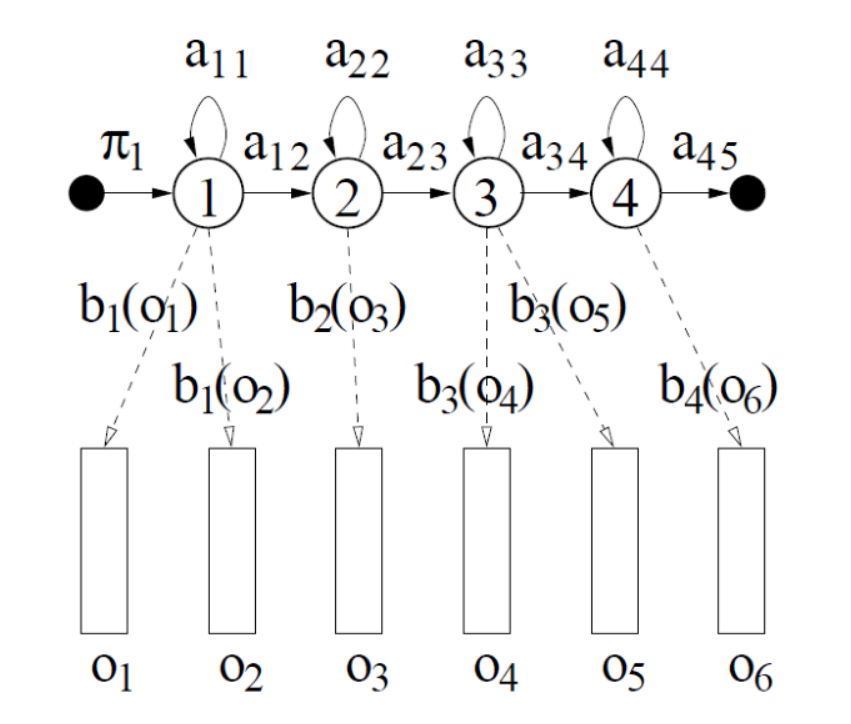
\includegraphics[width=0.5\linewidth]{images/hidden_markov.png}
    %\vspace{1em}
    \caption{Przykładowe reprezentacja Ukrytego Modelu Markowa. Prostokąty to obserwacje, kółka to stany ukryte.}
    \label{fig:pdgd}
    \source{M. Pietrzykowski. Wykład 4 - Ukryte Modele Markowa. \cite{Pietrzykowski2020}}
\end{figure}

\subsubsection{Mając sekwencję obserwacji $O = (O_1, O_2, \ldots, O_T)$ i model $\lambda = (A, B, \pi)$ jakie jest prawdopodobieństwo tej sekwencji pod warunkiem tego modelu, czyli $P(O|\lambda)$}

Prawdopodobieństwo $P(O|\lambda)$ musi być wyznaczone używając formuła na całkowite prawdopodobieństwo, tj. brać pod uwagę wszystkie możliwe ścieżki stanów. Takie przeszukiwanie w sposób zachłanny jest niemożliwe w praktyce. Złożoność obliczeniowa wynosi $O(TN^T)$\cite{Pietrzykowski2020}. 

W praktyce to zadanie rozwiązuje się za pomocą algorytmu \textbf{Forward-Backward}. Jego złożoność jest rzędu $O(TN^2)$\cite{Pietrzykowski2020}.

\subsubsection{Mając sekwencję obserwacji $O = (O_1, O_2, \ldots, O_T)$ i model $\lambda = (A, B, \pi)$ jak dobieramy najlepszą sekwencję stanów $Q = (q_1, q_2, \ldots, q_T)$, która odpowiada sekwencji obserwacji O?}

Mając sekwencję obserwacji należy odpowiedzieć jaka jest najbardziej prawdopodobna sekwencja stanów ukrytych uwzględniając model (tj. prawdopodobieństwa przejść oraz prawdopodobieństwa obserwacji).

Aby odpowiedzieć na to pytanie używamy algorytmu \textbf{Viterbiego} bazujący na metodach programowania dynamicznego. Jego celem jest znalezienie jednego najlepszej sekwencji stanów, która maksymalizuje $P(Q, O|\lambda)$~\cite{Pietrzykowski2020}.

\subsection{Mając sekwencję obserwacji $O = (O_1, O_2, \ldots, O_T)$ i znając tylko $M$ i $N$ (liczba obserwacji i stanów) jak stroić model?}

Jak dobrać najlepsze zmienne modelu $\lambda = (A, B, \pi)$ aby zmaksymalizować $P(O|\lambda)$?

Mamy sekwencję obserwacji, wiedząc ile ma być stanów i obserwacji jak nastroić model?

Jest to najtrudniejszy z problemów. W tym celu używa się podejścia iteracyjnego nazwanego \textbf{metodą Bauma-Welcha}~\cite{Pietrzykowski2020}.

% \subsection{Cechy obiektów audio i metody ekstrakcji cech tych obiektów}
% TODO
% Edward Półroliczak. Ekstrakcja cech.

% \subsection{Przebieg uczenia ze wzmocnieniem i pozyskiwana w tym procesie wiedza}
% TODO
% Marcin Pluciński. Uczenie maszynowe 2.

\subsection{Cechy charakterystyczne splotowych sieci neuronowych}
% Paweł Forczmański. Uczenie maszynowe 2.

\textbf{Convolution Neural Networks} (CNN, ConvNet) to wariant MLP inspirowany biologicznie, gdzie mnożenie wag i sygnału wejściowe zastąpione jest operacją \textbf{splotu} \cite{Forczmanski2020}.

Cechami charakterystycznymi splotowych sieci są:

\begin{itemize}
    \item rzadka reprezentacja
    \item współdzielone wagi
    \item pooling (zmniejszanie rozdzielczości, np. wybierając maksymalną wartość z danego sąsiedztwa)
\end{itemize}

Sieci te potrafią stopniowo filtrować różne części danych i wyostrzać ważne fragmenty w procesie dyskryminacji (rozpoznawanie/klasyfikacja wzorców) \cite{Forczmanski2020}.

Sieci splotowe są łatwiejsze do uczenia, gdyż zawierają mniej parametrów (wykorzystują te same wagi) niż typowe sieci neuronowe \cite{Forczmanski2020}. 

Wykorzystywanie głównie do obliczeń na strukturach dwuwymiarowych (np. obrazy) \cite{Forczmanski2020}.

\begin{figure}[H]
    \centering
    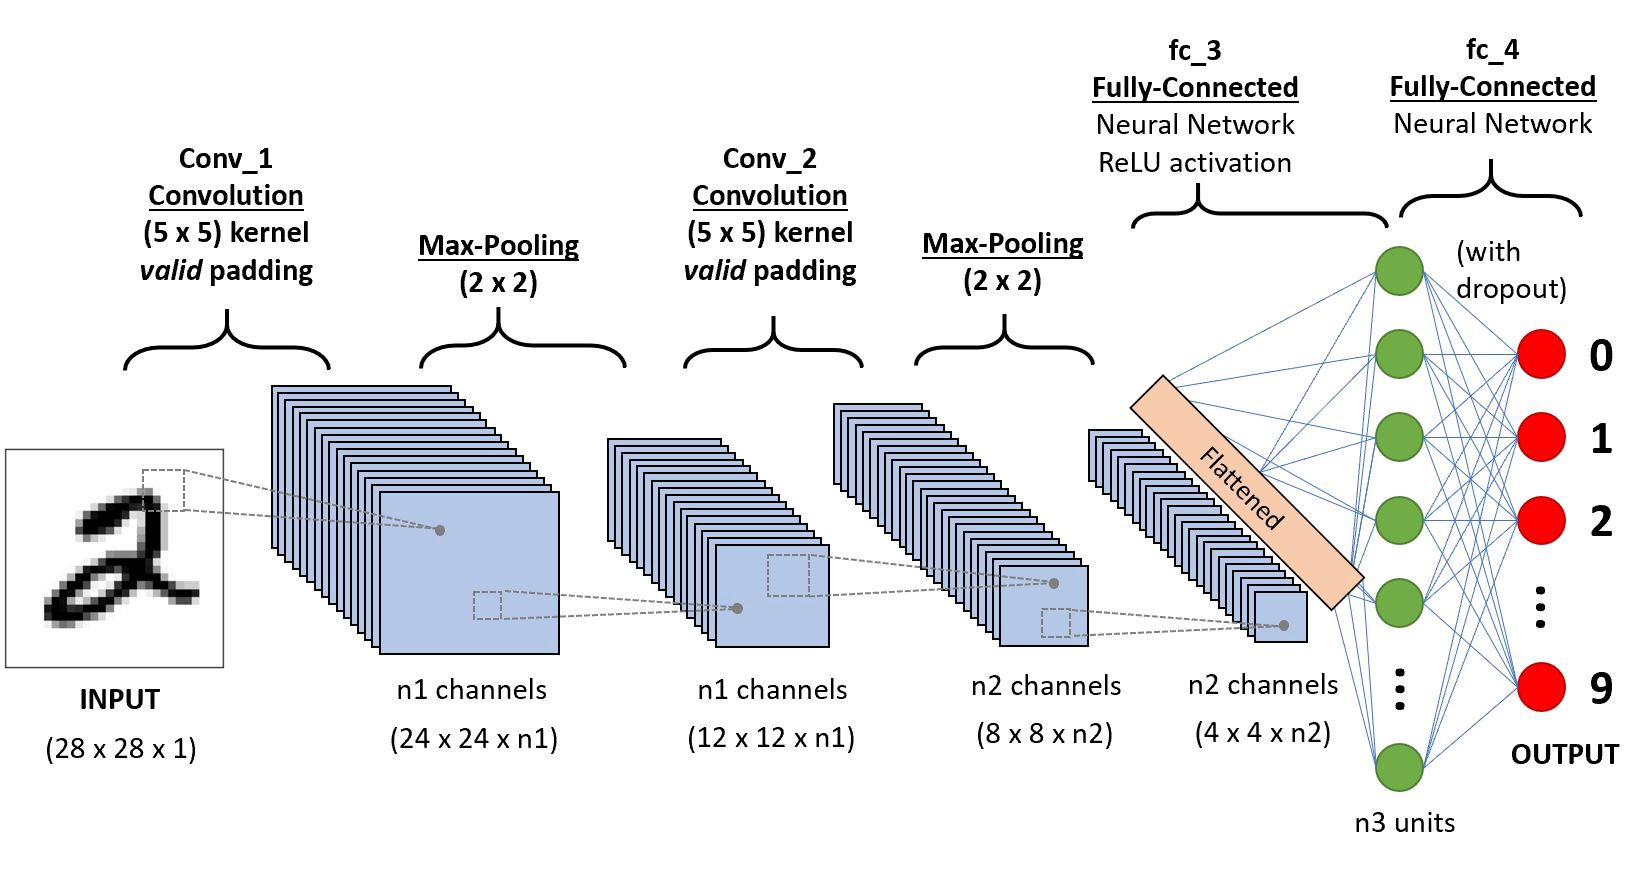
\includegraphics[width=0.7\linewidth]{images/cnn.jpeg}
    %\vspace{1em}
    \caption{Przykładowe architektura sieci splotowej.}
    \label{fig:cnn}
    \source{\url{https://datasciencepr.com/convolutional-neural-network/}}
\end{figure}

Pojedynczy neuron (jednostka obliczeniowa) w sieciach splotowych definiuje się za pomocą:

\begin{itemize}
    \item szerokości,
    \item wysokości,
    \item głębokości (liczba filtrów),
    \item stride (krok przesunięcia filtru) \cite{Forczmanski2020}.
\end{itemize}

% \subsection{Podstawowe różnice między sygnałem mowy a sygnałem muzycznym w dziedzinie częstotliwości}
% TODO
% Tomasz Mąka. Sygnały akustyczne.

\subsection{Metody próbkowania sieci złożonych}
% Jarosław Jankowski. Sieci złożone.

To jest dziwne, bo to pytanie z przedmiotu \emph{Duże zbiory danych}, które były przedmiotem wspólnym.

Próbkowanie i agregacja dają możliwość rozwiązaniem problemu bardzo dużych zbiorów grafowych. Przykładowo chcąc analizować sieć połączeń na Facebooku, reprezentowaną przez ponad 1 miliard węzłów, potrzebowalibyśmy 1TB pamięci aby zapisać same relacje w postaci grafu, bez atrybutów, etykiet i treści~\cite{Jankowski2020_probkowanie}. 

W próbkowaniu sieci informacja o węzłach jest pozyskiwana dopiero po pobraniu danej próbki, \textbf{struktura całej sieci nie jest znana}. Wymagana jest strategia eksploracji sieci i stopniowego powiększania próbki. Celem próbkowania jest stopniowa identyfikacja małego zbioru przedstawicieli węzłów i powiązań ze struktury sieciowej, przy posiadanej niewielkiej wiedzy o całej sieci. W skrócie jest to uogólnienie sieci, stworzenie modelu sieci, która zachowuje \textbf{niektóre właściwości} sieci pierwotnej~\cite{Jankowski2020_probkowanie}. 

Przy agregacji cała struktura sieci musi być znana apriori. Celem agregacji są miary, które umożliwiają opis własności sieci na poziomie ogólnym~\cite{Jankowski2020_probkowanie}. 

W próbkowaniu sieci homogenicznych (jednorodnych) wyróżniamy dwie główne strategie:

\begin{itemize}
    \item Wybór węzłów lub krawędzi o zadanych właściwościach
    \begin{itemize}
        \item Losowy wybór węzłów
        \item Na podstawie stopnia wierzchołka (prawdopodobieństwo proporcjonalne do stopnia)
        \item Na podstawie miary PageRank
    \end{itemize}
    \item Pobieranie próbek w procesie eksploracji
    \begin{itemize}
        \item Random Walk - rekurencyjnie wybierany losowo tylko jeden z sąsiadów
        \item Snowball sampling - rekurencyjnie włączamy $n$ sąsiadów
        \item Poszukiwanie wzorców
    \end{itemize}
\end{itemize}

W sieciach heterogenicznych (niejednorodnych) możemy skorzystać z \emph{multi-graph sampling}, pobierania próbek z zachowaniem rozkładu typów, próbkowania z zachowaniem relacji~\cite{Jankowski2020_probkowanie}.


% \subsection{Elementy składowe procesu klasyfikacji sygnałów akustycznych}
% TODO
% Tomasz Mąka. Sygnały akustyczne.

% \subsection{Model SVM (procedura uczenia, wariant liniowy i nieliniowy, przekształcenia jądrowe).}
% TODO
% Marcin Korzeń. Uczenie maszynowe 1.

\subsection{Sieci perceptronowe i metody uczenia perceptronu (warianty algorytmów uczenia, głosowanie, zastosowania)}
% Marcin Korzeń. Uczenie maszynowe 1.

Sieć perceptronowa składa się z pojedynczej warstwy neuronów. Jako funkcja aktywacji wykorzystywana jest bipolarna progowa funkcja aktywacji. Peceptron zbiega w skończonej liczbie iteracji do rozwiązania gdy dane są liniowo separowalne (twierdzenie Novikoffa). Do uczenia perceptronu wykorzystuje się regułę perceptronu \cite{Korzen2020_8}.

 Z matematycznego punktu widzenia wagi perceptronu tworzą wektor normalny, który określa prostą (w przypadku dwóch wejść) lub hiperpłaszczyznę decyzyjną \cite{wiki:Perceptron}.

\begin{figure}[H]
    \centering
    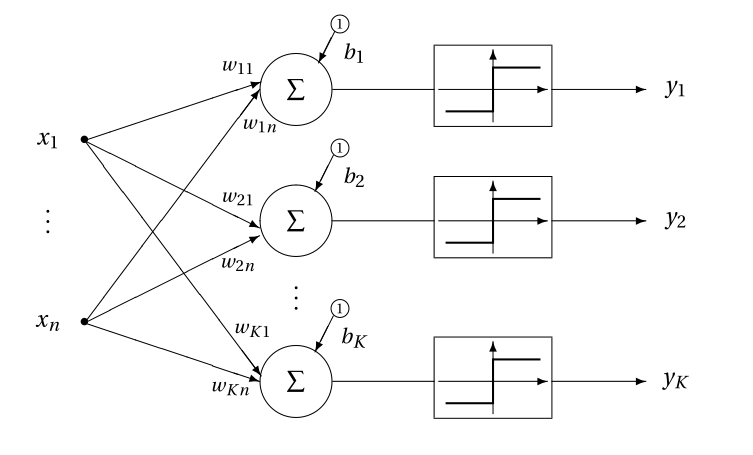
\includegraphics[width=0.5\linewidth]{images/perceptron.png}
    \caption{Wizualizacja perceptronu.}
    \label{fig:apriori}
    \source{Uczenie Maszynowe 1, Wykład VII - Perceptron \cite{Korzen2020_8}}
\end{figure}

Uczenie perceptronu przebiega zgodnie z \textbf{regułą perceptronu}. W skrócie, polega ona na korygowaniu wag w przypadku gdy próbka została źle sklasyfikowana. 

Inne warianty uczenia perceptronu to uczenie perceptronu z $\gamma$-marginesem, voted perceptron czy average perceptron.

Wariant z $\gamma$-marginesem polega na tym, że wagi są korygowane wtedy gdy próbka przekracza obrany margines (nie jak wcześniej czy jest źle klasyfikowana).

\textbf{Perceptron z głosowaniem} polega na tworzeniu wielu perceptronów (zestawów wag). Dla każdego zestawu wag przechowywany jest licznik, który opisuje ile próbek zostało dobrze sklasyfikowanych aż wagi należało poprawić. W procesie predykcji wybieramy głosem większościowym odpowiedzieć klasyfikatora. W \textbf{wersji average perceptron} różnica występuje tylko w odpowiedzi klasyfikatora. Gdzie wybierana jest średnia ze wszystkich klasyfikatorów.
\question




\subsection{Proces tworzenia zbioru uczącego, walidującego i testowego w głębokim uczeniu}
% Paweł Forczmański. Uczenie maszynowe 2.

Przygotowanie zbioru danych jest niezbędne w uczeniu maszynowym. Zbiór danych najczęściej jest podzielony na zbiór uczący, zbiór testowy i zbiór walidujący. 

Zbiór uczący jest wykorzystywany do uczenia modelu. Jest on największy ze wszystkich. Przede wszystkich w głębokim uczeniu wymagane są duże ilości próbek uczących.

Zbiór walidujący wykorzystywany jest do testowania na etapie tworzenia i implementacji modeli. Wykorzystywany jest to oceniania modeli z różnymi hyperparametrami. 

Zbiór testowy powinien zostać użyty tylko raz, na końcu całego procesu implementacji modelu. Wykorzystywany jest do przetestowania skuteczności stworzonego rozwiązania. 

W przypadku braku wystarczającej liczby danych uczących można korzystać z kroswalidacji. Wykorzystuje się ją najczęściej w metodach klasycznych. W głębokim uczeniu metoda kroswalidacji nie jest wykorzystywana ze względu na długie czasy uczenia modeli.

W głębokim uczeniu rozmiar próby uczącej powiększa się za pomocą augmentacji. W przypadku obrazów może to być odbijanie w poziomie, rozjaśnianie, kadrowanie, itd.

\subsection{Sposób działania algorytmów uczących AdaBoost i RealBoost}
% Przemysław Klęsk. Uczenie maszynowe 2.

Algorytmy z rodziny boosting polegają na reważeniu przykładów uczących. Ich zasadniczą cechą jest odporność na przeuczenie.

Klasyfikator boosting składa się z wielu słabych klasyfikatorów. Najczęściej łączy się je z \emph{decision stump} - bardzo zdegenerowane drzewa decyzyjnego, lub innymi wariantami klasyfikatorów (drzewa decyzyjne, SVM, naiwny Bayes) \cite{Klesk2020}.

Uczenie klasyfikatora składa się z wielu rund. W każdej iteracji uczony jest słaby klasyfikator na danych uczących używając ważonych przykładów. Wagi przykładów aktualizuje się tak, że najważniejsze stają się próbki źle sklasyfikowane \cite{Klesk2020}.

W pojedynczej rundzie wybór słabego klasyfikatora odbywa się teoretycznie według dowolnego obranego kryterium błędu. Najczęściej rozważa się minimalizację błędu klasyfikacji lub minimalizację kryterium wykładniczego \cite{Klesk2020}.

Wystarczy że słabe klasyfikatory będą dawać odpowiedzi różne od 0.5. Gdy dokładność klasyfikatora jest mniejsza niż 0.5 to odpowiedź klasyfikatora jest negowana.

Rozwinięciem AdaBoost jest RealBoost. Słabe klasyfikatory są rzeczywistoliczbowe a nie binarne jak w Adaboost. Odpowiedź słabego klasyfikatora jest zwykle ustalana jako przybliżenie połowy przekształcenia logit. Rezygnuje się ze współczynników ważących słabe klasyfikatory. Mechanizm ważenia klasyfikatorów jest wpleciony w same odpowiedzi rzeczywistoleiczbowe \cite{Klesk2020}.
\question


\subsection{Omówienie na przykładzie algorytmu Apriori odkrywania asocjacji w zbiorach danych}
% Joanna Kołodziejczyk. Eksploracja danych.

Algorytm Apriori opiera się na własności, że wszystkie podzbiory częstego zbioru przedmiotów również muszą być częste. Przykładowo, w transakcjach często występuje reguła: bułka, ser żółty, pomidor $\rightarrow$ szynka, to wszystkie elementy tej reguły też często występują w zbiorze transakcji \cite{Kolodziejczyk2020}.

Algorytm Apriori jest przeznaczony do znajdowania wzorców w dużych zbiorach danych. Jeśli jakieś wzór występuje często, to jest on uważany za ,,interesujący'' \cite{Kolodziejczyk2020}.

Algorytm składa się z dwóch etapów: znajdowania częstych wzorców z wykorzystaniem progu minimalnego wsparcia, oraz znajdowaniem odpowiednich reguł z progiem minimalnego zaufania. Generowanie kandydatów do wzorców można przeprowadzić metodą brute-force, albo metodami $F_{k-1} \times F_1$, lub $F_{k-1} \times F_{k-1}$. Metoda brute-force nie sprawdzi się w bardzo dużych zbiorach danych.

\begin{figure}[H]
    \centering
    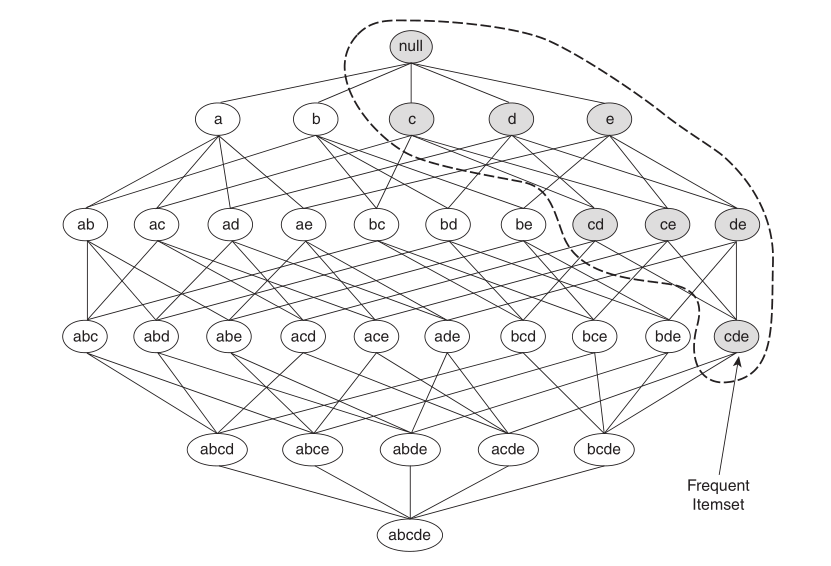
\includegraphics[width=0.5\linewidth]{images/apriori.png}
    \caption{Przedstawienie reguły Apriori. Jeżeli zbiór $\{c, d, e\}$ jest częsty, to wszystkie podzbiory też są częste.}
    \label{fig:apriori}
    \source{\url{https://www-users.cs.umn.edu/~kumar001/dmbook/ch5_association_analysis.pdf}}
\end{figure}


Na początku tworzymy zbiór potencjalnych wzorców jednoelementowych z danym progiem wsparcie. Wyszukiwanie przeprowadzamy iteracyjnie zwiększając wielkości zbiorów. 

Mając wygenerowane potencjalne wzorce z pierwszego kroku należy wygenerować reguły z zaufaniem większym niż ustalony minimalny próg wsparcia. Wygenerowane reguły należy posortować malejąco na podstawie metryki \emph{lift}.

\subsection{Przykład siedzi bayesowskiej (przekonań): struktura sieci, właściwości i jej interpretacja oraz uczenie}
% Joanna Kołodziejczyk. Eksploracja danych.

Sieć Bayesowska (sieć przekonań) jest probabilistycznym modelem grafowym, który reprezentuje zbiór zmiennych i ich zależności warunkowych za pomocą acyklicznego grafu. Sieci Bayesowskie są dobre do przewidywania zdarzeń zależnych (obliczania \emph{likelihood} \cite{wiki:Likelihood_function}) na podstawie zdarzenia zaobserwowanego 
\cite{wiki:Bayesian_network}. Przykładowo mamy sieć przedstawioną na rysunku \ref{fig:bayesian}. Na podstawie różnych przesłanek Holmes ma zdecydować czy wracać do domu z powodu włamania. Są to: alarm, telefon od Watsona, trzęsienie ziemi i informacja w wiadomościach o trzęsieniu.


\begin{figure}[H]
    \centering
    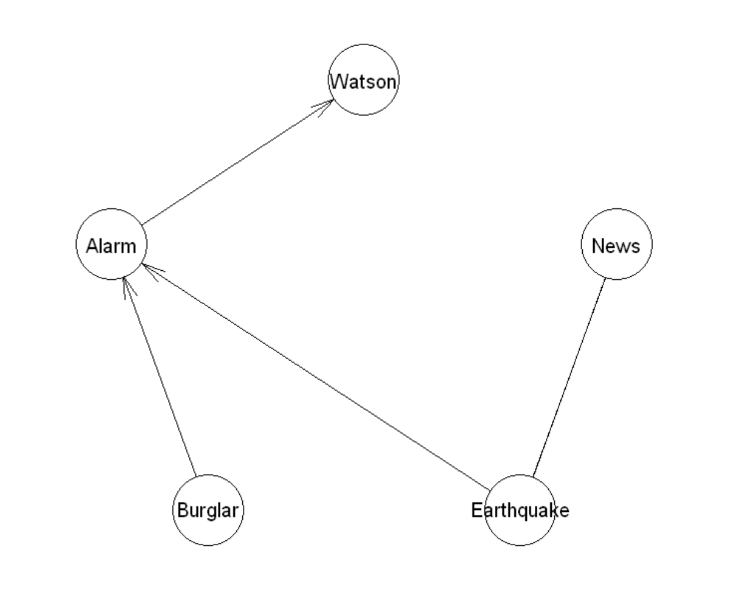
\includegraphics[width=0.5\linewidth]{images/bayesian.png}
    \caption{Przykład sieci Bayesowskiej}
    \label{fig:bayesian}
    \source{Opracowanie własne}
\end{figure}


Na laboratorium wykorzystywaliśmy bibliotekę \emph{bnlearn}\footnote{\url{https://www.bnlearn.com/documentation/man/bn.fit.html}} do tworzenia sieci i ich uczenia. Aby nauczyć sieć wprowadzaliśmy prawdopodobieństwa warunkowe zdarzeń.
\question

\subsection{Deskryptory cech niskopoziomowych - wybrane algorytmy w odniesieniu do wykorzystywanych cech}
% Dariusz Frejlichowski. Ekstrakcja cech.

Deskryptory cech odnoszą się do zagadnienia ekstrakcji cech. Deskryptor opisuje daną cechę za pomocą wartości numerycznych. Poniżej opisywano tylko deskryptory odnoszące się do obrazów. Oprócz tego istnieją inne deskryptory, np. w rozpoznawaniu dźwięku częstotliwość fundamentalna, formanty, itd.

\textbf{Atrybuty niższego poziomu abstrakcji} - metadane typu sygnałowego, są wartościowane przez komputer (np. kolor dominujący, histogram krawędzi, aktywność ruchu w obrazie, czy linia melodyczna utworu muzycznego) \cite{Frejlichowski2020}.

Standard MPEG-7 opisuje między innymi deskryptory wizualne. Deskryptory wizualne MPEG-7 opisują na \textbf{niewielu} bitach obrazy, sekwencje obrazów, obszary w obrazie itd. 

Deskryptor powinien być:

\begin{itemize}
    \item efektywny i ekspresyjny (porównywalny z widzeniem u ludzi),
    \item zwarty (w aspekcie pamięci),
    \item o małej złożoności ekstrakcji i zapytań \cite{Frejlichowski2020}.
\end{itemize}

Wyróżniamy następujący podział deskryptorów:

\begin{itemize}
    \item \textbf{Koloru} - Scalable Color, Color Structure, Dominant Color, histogramy,
    \item \textbf{Kształtu} - sygnatura, UNL, UNL-F, mUNL,
    \item \textbf{Odcieni szarości} - Polar-Fourier Greyscale Descriptor, Rzutowanie wartości,
    \item \textbf{Ruchu},
    \item \textbf{Tekstury}.
\end{itemize}

\subsubsection{Deskryptory kształtu}

Główne problemy z deskryptorami kształtu to:

\begin{itemize}
    \item obrót, skalowanie, przesunięcie (przekształcenia afiniczne)
    \item szum,
    \item nieciągłości,
    \item okluzja.
\end{itemize}

Czyli najlepszy deskryptor jest inwariantny względem obrotu, skalowania, przesunięcia oraz jest niewrażliwy na szum i okluzję.

Proste deskryptory kształtu to m.in. pole powierzchni, długość obwodu, kołowość, zwartość, mimośród, powłoka wypukła, object aspect ratio, itd. \cite{Frejlichowski2020_2}

Przykładowym deskryptorem jest UNL-F. Zapewnia on dobrą odporność na szum, przekształcenia afiniczne (transformata Fouriera daje odporność na obrót). Jedyną wadą jest brak odporności na okluzję. W pewnym stopniu rozwiązuje to mUNL, który zmienia podejście do wyznaczania centroidu  \cite{Frejlichowski2020_2}.

W skrócie UNL-F składa się on z następujących kroków:

\begin{enumerate}
    \item Binaryzacja obiektu
    \item Wyznaczenie centroidu
    \item Przekształcenie do współrzędnych polarnych
    \item Wycinek widma po transformacie 2D Fouriera -- tego kroku nie ma w zwykłej metodzie UNL
\end{enumerate}

\begin{figure}[H]
    \centering
    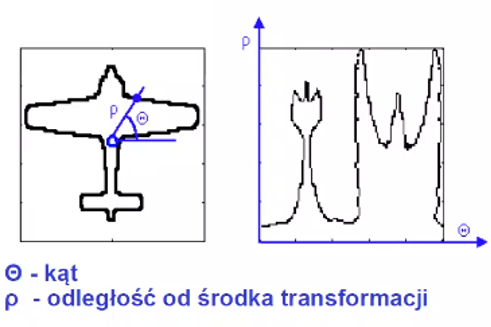
\includegraphics[width=0.5\linewidth]{images/unl.png}
    \caption{Działanie deskryptora UNL}
    \label{fig:unl}
    \source{Wykład 2 - D. Frejlichowski \cite{Frejlichowski2020_2}}
\end{figure}

\subsubsection{Deskryptory koloru}

Przykładowe deskryptory koloru ze standardu MPEG-7 to:

\begin{itemize}
    \item Deskryptor koloru dominującego
    \item Skalowalny deskryptor koloru
    \item Deskryptor GOF i GOP
    \item Deskryptor struktury koloru
    \item Deskryptor widoku koloru (layout)
    \item Temperatura barwowa \cite{Frejlichowski2020_6}
\end{itemize}

Inne deskryptory koloru to:

\begin{itemize}
\item histogram RGB lub HSV - może dawać takie same wyniki dla różnych obrazów
\item IBOX8
\item DHV
\item RGBBOX8
\item RGBI \cite{Frejlichowski2020_6}
\end{itemize}

Przykładowo, deskryptor koloru dominującego polega na wyznaczenie $n$ kolorów dominujących dla obrazu za pomocą algorytmu $k$-means i obliczenie ich udziałów \cite{Frejlichowski2020_6}.

Skalowalny deskryptor koloru bazuje na przestrzeni barw HSV i transformacji Haara zastosowanej na wartościach histogramu koloru \cite{Frejlichowski2020_6}.

Deskryptor rozkładu koloru (Color Layout Descriptor) uchwyca rozkład przestrzenny kolorów w bazie. Polega na transformacji DCT dla poszczególnych składowych w przestrzeni YcbCr~\cite{Frejlichowski2020_6}.

\subsubsection{Deskryptory odcieni szarości}

W pewnym sensie deskryptory odcieni szarości łączą w sobie deskryptory kolorów i kształtu. Przykładowym deskryptorem jest Polar-Fourier Grayscale Descriptor.

Polega on na wstępnym preprocessingu (filtry), wyznaczeniu centroidu obrazu w skali szarości, transformacji obrazu do współrzędnych biegunowych i wycięciu fragmentu widma po transformacie 2D Fouriera \cite{frejlichowski2015application}.

Alternatywny deskryptor polegał na przekształceniu biegunowym i rzutowaniu wartości. Rzutowanie to suma po kolumnach i suma po wierszach. Taki deskryptor daje na wyjściu dwa wektory. Dawał gorsze wyniki niż PFGD \cite{Frejlichowski2020_5}.


\subsection{Główne miary centralności w sieciach złożonych}
% Jarosław Jankowski. Sieci złożone.

Sieci złożone to nic innego jak rozbudowane grafy służące np. do modelowania społeczności, węzłów komunikacyjnych, infrastruktury itd. Mogą występować grafy skierowane lub nieskierowane.

\textbf{Miary centralności} wyznaczają najważniejsze węzły w grafie ze względu na różne własności~\cite{Jankowski2020}. Wyróżniamy następujące miary:

\begin{itemize}
    \item Degree - stopień wierzchołka
    \item Betweenness - ile razy węzeł stanowi pomost jako element najkrótszej ścieżki pomiędzy innymi węzłami sieci
    \item Closeness - średnia długość najkrótszej ścieżki między węzłem, a wszystkimi innymi węzłami. Bardziej centralne węzły mają bliżej do wszystkich innych węzłów w sieci.
    \item PageRank - zliczanie liczby i jakości linków do węzłów aby określić ważność węzła. Podstawowym założeniem jest to, że ważne węzły otrzymują więcej połączeń z innych ważnych węzłów.
    \item Eigenvector
\end{itemize}

\subsection{Pakiety języka Python wykorzystywane w analizie danych}
% Marcin Pluciński. Języki analizy danych.

Najpopularniejsze pakiety Pythona wykorzystywane w analizie danych to:

\begin{itemize}
    \item \textbf{numpy} - wielowymiarowe macierze i operacje na tych strukturach
    \item \textbf{scipy} - optymizacja, algebra liniowa, interpolacja, FFT, przetwarzanie sygnałów itd.
    \item \textbf{pandas} - przetwarzanie danych i analiza. Struktury danych do manipulowania tabelami i szeregami czasowymi.
    \item \textbf{matplotlib} - biblioteka do wizualizacji
    \item \textbf{geopandas} - odpowiednik pandas (rozszerzenie) do danych przestrzennych
    \item \textbf{sklearn} (scikit learn) - implementacje modeli uczenia maszynowego
\end{itemize}

\subsection{Techniki regularyzacji modeli klasyfikacyjnych i regresyjnych (regularyzacja L1, L2, elastic net; problemy optymalizacyjne; zastosowania)}
% Marcin Korzeń. Uczenie maszynowe 1.

Ogólne podejście do problemu uczenia można zdefiniować następująco:

\begin{equation}
    Q(\theta \mid \mathscr{D})=L(\theta \mid \mathscr{D})+\gamma R(\theta)
\end{equation}

gdzie:

\begin{description}
\item[L(\theta \mid \mathscr{D})] to funkcja straty, błędu, dopasowanie modelu do danych,
\item[R(\theta)] to kara za złożoność modelu,
\item[\gamma] ustala kompromis pomiędzy dopasowaniem, a złożonością.
\end{description}

Regularyzacja to modyfikacja modelu, np. przez dodanie kary za złożoność, która ma na celu zmniejszenie błędu testowego zapobiegając zjawisku przeuczenia \cite{wiki:Regularization}.

Regularyzacja jest konieczna gdy:

\begin{itemize}
    \item mamy pewną wiedzę na temat możliwych rozwiązań,
    \item niejednoznaczność rozwiązania,
    \item numeryczna niestabilność algorytmów \cite{Korzen2020_12}.
\end{itemize}
\question

\textbf{Regularyzacja typu $L^1$ (lasso)} w modelach klasyfikacyjnych i regresyjnych stosujemy aby poprawić własności numeryczne algorytmów oraz gdy zależy nam na selekcji zmiennych w trakcie uczenia. Modele z taką regularyzacją są rzadkie, to znaczy, współczynniki przy wielu atrybutach są zerowe. Jest to zjawisko dobre w przypadku, gdy chcemy dokonać selekcji zmiennych -- mało jest atrybutów istotnych i dużo szumu.

\textbf{Regularyzacja typu $L^2$ (ridge)} w modelach klasyfikacyjnych i regresyjnych również sotsujemy aby poprawić własności numeryczne algorytmów oraz w przypadkach, gdy dane zawierają wiele zmiennych skorelowanych.

Model ElasticNet łączy regularyzację $L^1$ oraz regularyzację $L^2$ \cite{wiki:Elastic_net_regularization}. 

Nie wiem jakie są problemy optymalizacyjne tych technik regularyzacji.
\question

Podsumowując:

\begin{itemize}
    \item składnik straty $L(\theta \mid \mathscr{D})$ jest mniej istotny,
    \item składnik związany z regularyzacją $R(\theta)$ prowadzi do różnych jakościowo modeli,
    \item $L^1$ jest dobry, gdy mało jest atrybutów istotnych i dużo szumu (bardzo dobry mechanizm selekcji), oraz gdy jest mało danych,
    \item $L^2$ jest dobry, gdy dużo jest atrybutów istotnych i dużo korelacji \cite{Korzen2020_12}.
\end{itemize}

\printbibliography[heading=bibintoc]

\appendix

\section{Przykłady do kopiowania}

\begin{table}[H]
\caption{Czas trwania jednej epoki dla rozmiaru obrazu}
\vspace{1em}
\centering
\begin{tabular}{@{}lr@{}}
\toprule
Rozmiar          & Czas {[}s{]} \\ \midrule
$32 \times 32$   & 0.1288       \\
$64 \times 64$   & 0.2000       \\
$128 \times 128$ & 1.046        \\ \bottomrule
\end{tabular}
\end{table}

\code{Przykład kodu}
{Opracowanie własne}{\label{kod:przyklad}}
\begin{lstlisting}[language=Python]
discriminator = make_discriminator_model()
generator = make_generator_model()
\end{lstlisting}

\begin{figure}[H]
    \centering
    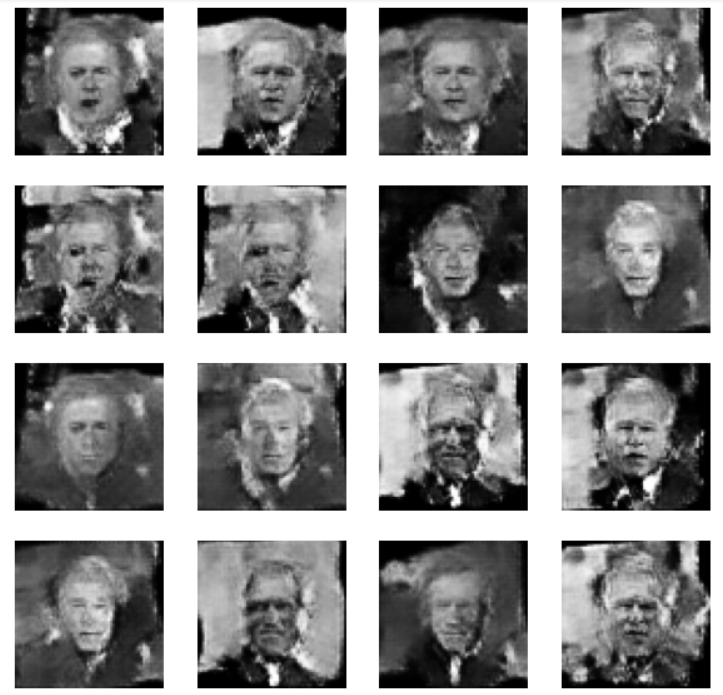
\includegraphics[width=0.7\linewidth]{images/sample.png}
    %\vspace{1em}
    \caption{Przykładowy obrazek}
    \label{fig:pdgd}
    \source{Opracowanie własne}
\end{figure}


\end{document}
